\documentclass[11pt]{article}
\usepackage{graphicx}
\usepackage{color}
\usepackage{comment}
\usepackage{multirow}
\usepackage{askmaps}
\usepackage{amssymb}
\usepackage{amsmath}

% Wrap long URLs with hyphens
\PassOptionsToPackage{hyphens}{url}\usepackage{hyperref}
\usepackage{pdftexcmds}
\usepackage{upquote}
\usepackage{textcomp}
\usepackage{minted}
\usepackage[listings]{tcolorbox}
\usepackage{enumerate}
\usepackage{enumitem}
\usepackage{mathtools}
\DeclarePairedDelimiter{\ceil}{\Big\lceil}{\Big\rceil}

\tcbset{
texexp/.style={colframe=black, colback=lightgray!15,
         coltitle=white,
         fonttitle=\small\sffamily\bfseries, fontupper=\small, fontlower=\small},
     example/.style 2 args={texexp,
title={Question \thetcbcounter: #1},label={#2}},
}

\newtcolorbox{texexp}[1]{texexp}
\newtcolorbox[auto counter]{texexptitled}[3][]{%
example={#2}{#3},#1}

\setlength{\topmargin}{-0.5in}
\setlength{\textheight}{9in}
\setlength{\oddsidemargin}{0in}
\setlength{\evensidemargin}{0in}
\setlength{\textwidth}{6.5in}

% Useful macros
\newenvironment{tightlist}
{\begin{itemize}
 \setlength{\parsep}{0pt}
 \setlength{\itemsep}{-2pt}}
{\end{itemize}}

\newenvironment{titledtightlist}[1]
{\noindent
 ~~\textbf{#1}
 \begin{itemize}
 \setlength{\parsep}{0pt}
 \setlength{\itemsep}{-2pt}}
{\end{itemize}}

% Change spacing before and after section headers
\makeatletter
\renewcommand{\section}
{\@startsection {section}{1}{0pt}
 {-2ex}
 {1ex}
 {\bfseries\Large}}
\makeatother

\makeatletter
\renewcommand{\subsection}
{\@startsection {subsection}{1}{0pt}
 {-1ex}
 {0.5ex}
 {\bfseries\normalsize}}
\makeatother

% Reduce likelihood of a single line at the top/bottom of page
\clubpenalty=2000
\widowpenalty=2000

% Other commands and parameters
\pagestyle{myheadings}
\setlength{\parindent}{0in}
\setlength{\parskip}{10pt}

% Commands for register format figures.
\newcommand{\instbit}[1]{\mbox{\scriptsize #1}}
\newcommand{\instbitrange}[2]{\instbit{#1} \hfill \instbit{#2}}

\graphicspath{{./figs/}}

\begin{document}
\def\PYZsq{\textquotesingle}


\title{EE219C HW1: SAT and BDDs}
\author{Vighnesh Iyer}
\date{}
\maketitle

\section{Horn-SAT and Renamable Horn-SAT}
\begin{enumerate}[label=(\alph*)]
    \item {\color{blue}Recall from class that a HornSAT formula is a CNF formula in which each clause contains at most one positive literal. Give an algorithm to decide the satisifiability of HornSAT formulas in linear time (in the number of variables $n$).}

    We can write a HornSAT clause as an implication:
    \begin{align*}
        \text{In general: } &A \rightarrow B \iff \neg A \lor B \\
        \text{HornSAT Clause: } &x_p \lor \neg x_{n,1} \lor \neg x_{n,2} \lor \dots \lor \neg x_{n,l} \\
        \text{Group terms: } &(\neg x_{n,1} \lor \neg x_{n,2} \lor \dots \lor \neg x_{n,l}) \lor x_p \\
        \text{Let A = } &(\neg x_{n,1} \lor \neg x_{n,2} \lor \dots \lor \neg x_{n,l}) \\
        \text{Let B = } &x_p \\
        \neg A =& (x_{n,1} \land x_{n,2} \land \dots \land x_{n,l}) \\
        \text{Conclude: } &x_p \lor \neg x_{n,1} \lor \neg x_{n,2} \lor \dots \lor \neg x_{n,l} \iff (x_{n,1} \land x_{n,2} \land \dots) \rightarrow x_p
    \end{align*}

    We can also handle special-case HornSAT clauses by converting them to implications:
    \begin{enumerate}
        \item Unit positive literal clause
            \begin{align*}
                x_p \iff (\mathbf{T} \rightarrow x_p)
            \end{align*}
            i.e. for the CNF formula to be SAT, $x_p$ must be set to $\mathbf{T}$.
        \item No positive literals in the clause
            \begin{align*}
                (\neg x_{n,1} \lor \dots \lor \neg x_{n,l}) \iff ((x_{n,1} \land \dots \land x_{n,l}) \rightarrow \mathbf{F})
            \end{align*}
    \end{enumerate}

    Note that if no unit positive literal clauses are present, the formula is immediately satisfiable with the assignment of all variables to $\mathbf{F}$, since the implication $\mathbf{F} \rightarrow \mathbf{F}$ is true.

    HornSAT can only be unsat if there is at least one unit positive literal clause. In this case, we can selectively flip variables to true based on the implications and find the formula is unsat if flipping a variable would contradict a previous assignment.
\end{enumerate}

\section{The Pigeon-Hole Problem}
\begin{enumerate}[label=(\alph*)]
    \item {\color{blue} Encode the pigeon-hole problem as DIMACS CNF for $n = 4, 5, 6, \dots, 15$. Run it with MiniSAT and plot how the runtimes vary with $n$. Describe your observations.}

    I wrote a \href{https://github.com/vighneshiyer/ee219c-formal/blob/master/formal-toolkit/src/main/scala/formal/PigeonHoleProblem.scala}{package in Scala} to handle CNF formulas. Here's the relevant exerpt, which returns the pigeon-hole problem as CNF for $n$ pigeons:

        \begin{minted}[breaklines]{scala}
def problem(n: Int): CNFFormula = {
val pigeons = 1 to n
val holes = 1 until n
// stride on pigeons with stride size of holes
def pigeonHoleToVariable(p: Int, h: Int): Int = {
  (p-1)*holes.size + h
}
val everyPigeonInOneHole: CNFFormula = pigeons.map {
  p => holes.foldLeft(Set.empty[Int]) {
    case (s, h) => s.union(Set(pigeonHoleToVariable(p, h)))
  }
}.toSet
val noTwoPigeonsPerHole = holes.foldLeft(Set.empty[Set[Int]]) {
  case (ss, h) => ss.union(pigeons.combinations(2).foldLeft(Seq.empty[Set[Int]]) {
    case (s, p) => s :+ Set(-pigeonHoleToVariable(p(0), h), -pigeonHoleToVariable(p(1), h))
  }.toSet)
}
everyPigeonInOneHole.union(noTwoPigeonsPerHole)
}
        \end{minted}

        I wrote a script to run MiniSAT on the produced CNF file and plotted the runtimes (with a 60 second timeout):

        \begin{figure}[H]
          \centering
          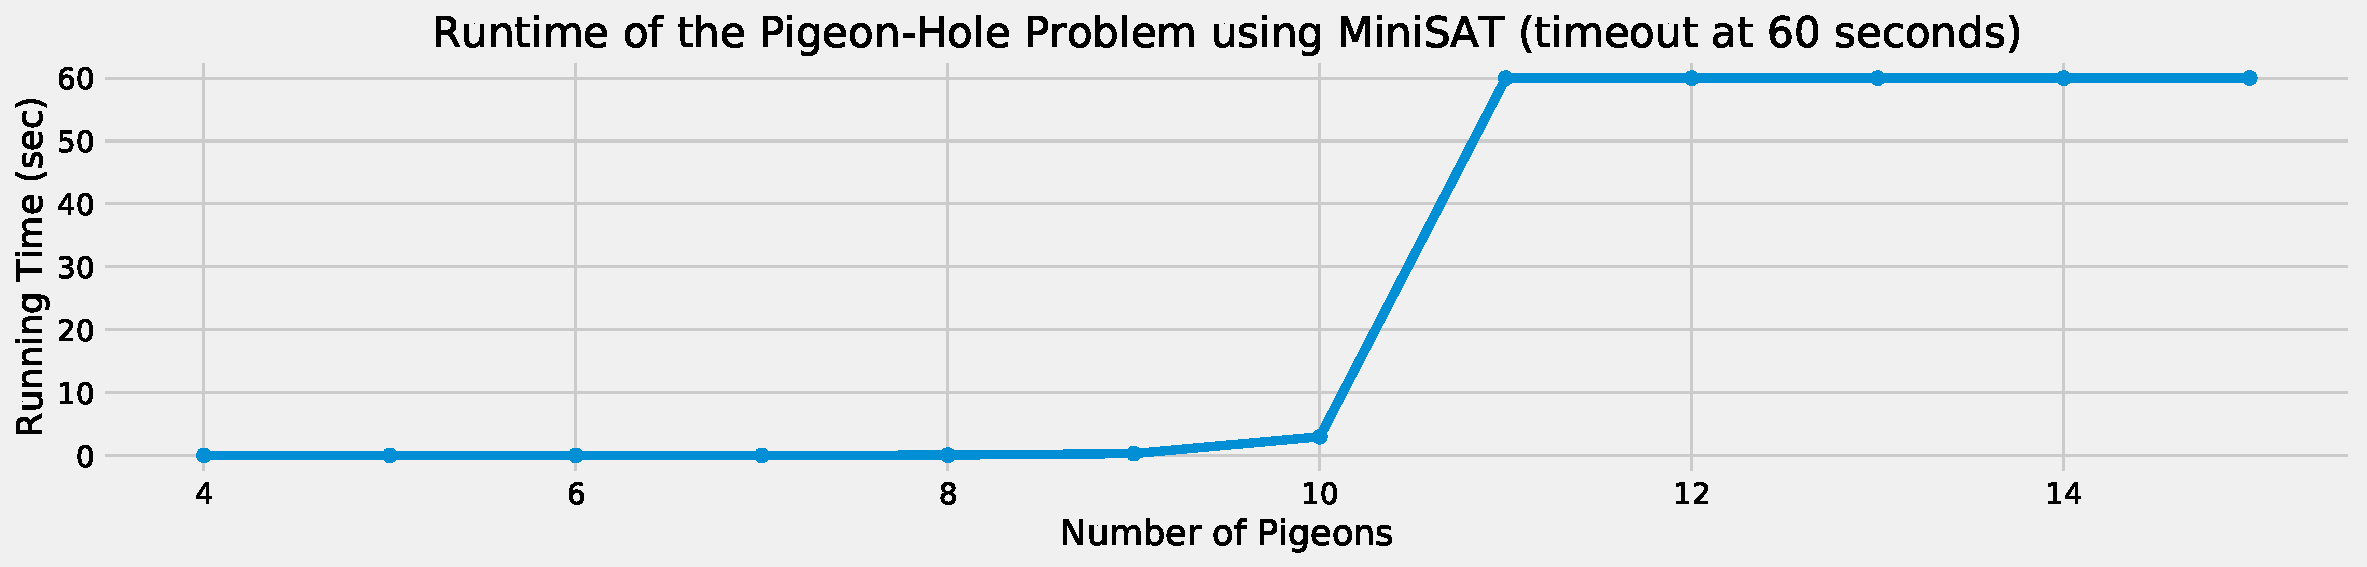
\includegraphics[width=\textwidth]{figs/pigeon_hole_runtime.pdf}
        \end{figure}

        There is a noticable increase in runtime for 10 pigeons, and 11+ pigeons require more than 1 minute of runtime. The runtime growth is exponential. This is clear if plotted on a log-scale:

        \begin{figure}[H]
          \centering
          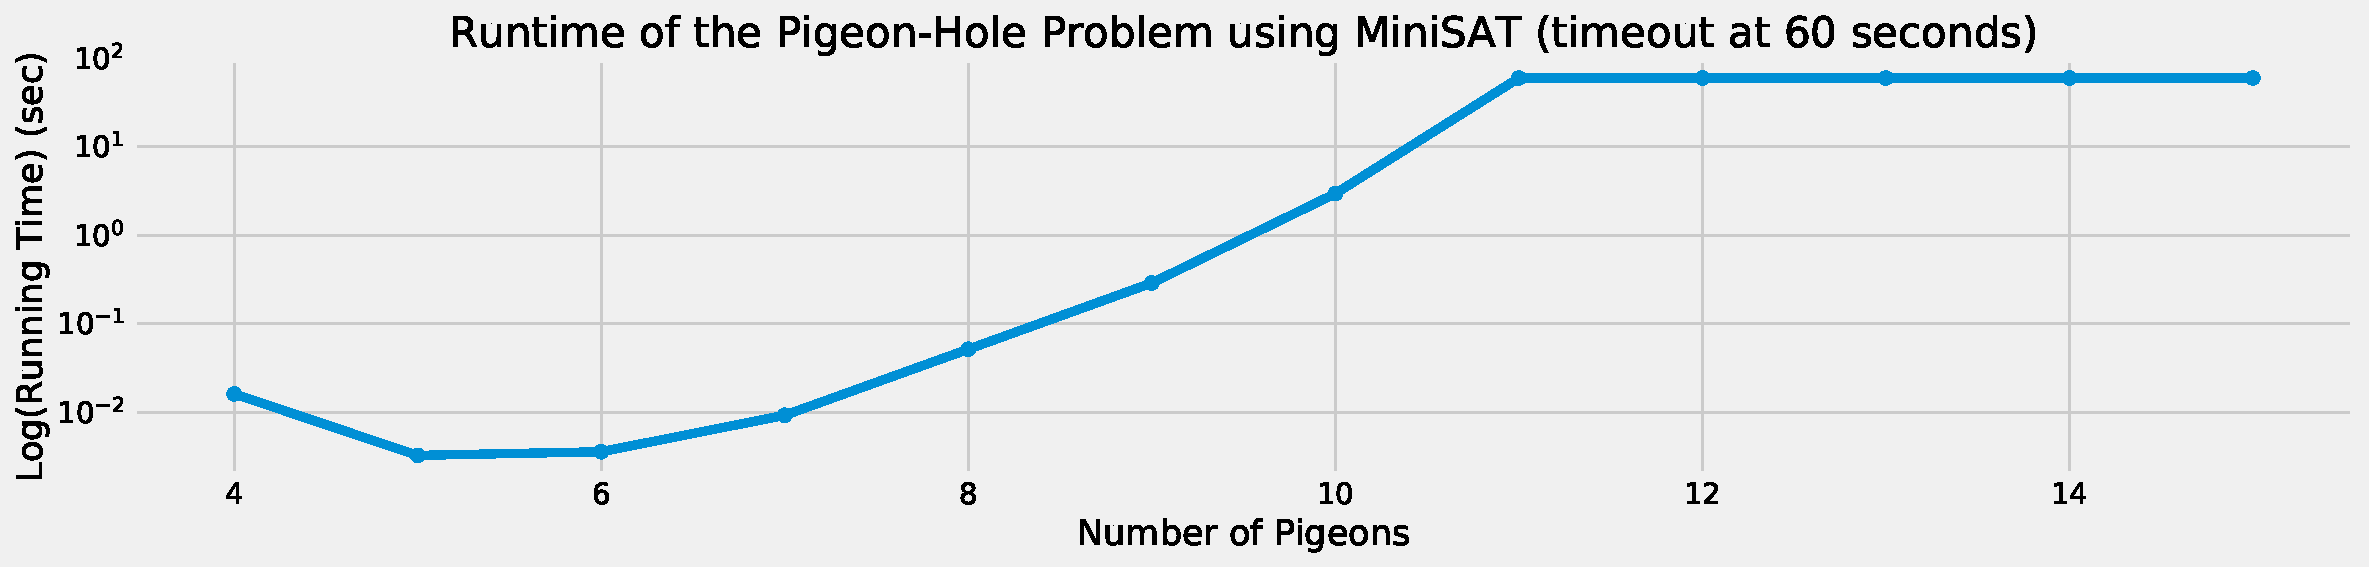
\includegraphics[width=\textwidth]{figs/pigeon_hole_runtime_log.pdf}
        \end{figure}

    \item {\color{blue} Construct the BDD for the pigeon-hole problem and verify it simplifies to false. What happens when you increase $n$? Does the variable order matter? Use the Python \texttt{dd} package.}

      \begin{minted}[breaklines,tabsize=2]{python}
def pigeonhole(pdfname, n):
    print ('  [Pigeonhole Problem for n=%d]' % n)

    bdd = _bdd.BDD()
    for p in range(n):
        for h in range(n-1):
            bdd.declare('x_%d_%d' % (p, h))

    # All pigeons are in at least 1 hole
    all_in_a_hole = map(lambda p: reduce(lambda x, y: x | y, [bdd.var('x_%d_%d' % (p, h)) for h in range(n-1)]), range(n))
    all_in_a_hole = reduce(lambda x, y: x & y, all_in_a_hole)

    # No 2 pigeons are in the same hole
    no_two_in_same_hole = [~(bdd.var('x_%d_%d' % (c[0], h))) | ~(bdd.var('x_%d_%d' % (c[1], h))) for c in itertools.combinations(range(n), 2) for h in range(n-1)]
    no_two_in_same_hole = reduce(lambda x, y: x & y, no_two_in_same_hole)
    f = all_in_a_hole & no_two_in_same_hole
    if (f == bdd.true):
        print('SAT')
    else:
        print('UNSAT')
      \end{minted}
\end{enumerate}
\end{document}
